\section{Some Synthetic Results}\label{app:dttts.experiments}
In this part, we give some synthetic experimental results comparing \DTTTS to \Hyperband and to \texttt{SHA}, a state-of-the-art algorithm for finite BAI that can be adapted to the infinite setting. In those experiments, the arms are Bernoulli distributed and the reservoir distribution $\nu_0$ is fixed to some $\text{Beta}(a,b)$ distribution. 

Infinite Sequential Halving (\ISHA) consists in running \texttt{SHA} on a fixed number of arms drawn from the reservoir. Observe that for a total budget $B$, there exists a maximum number of arms $K^\star$ that can be processed by \texttt{SHA}, which satisfies $B = \ceil{K^\star\log_2(K^\star)}$. Following~\cite{aziz2018infinite}, we run \ISHA with $K^\star$ arms drawn from the reservoir. % seems to be empirically performing better than \Hyperband.

We report in Fig.\,\ref{fig:dttts} the simple regret as a function of time for different algorithms and four Beta reservoir distributions. $\HTTTS$ and $\DTTTS$ are run with $\beta=1/2$ which is known to be a robust choice \citep{russo2016ttts}. Each point represents the expected simple regret $\mathbb{E}[1 - \mu_{I_n^*}]$ estimated over 1000 replications for an algorithm run with budget $n$. \DTTTS is very competitive on 3 reservoirs and \HTTTS is sometimes better, sometimes worse than \Hyperband. We also tried the \SiRI algorithm \citep{carpentier2015siri} (with $b$ as the tail parameter when $\nu_0=$Beta$(a,b)$) but obtained worse performance and therefore do not report the results.

\begin{figure}[ht]
  \centering
  \begin{subfigure}[t]{0.2\textwidth}
    \centering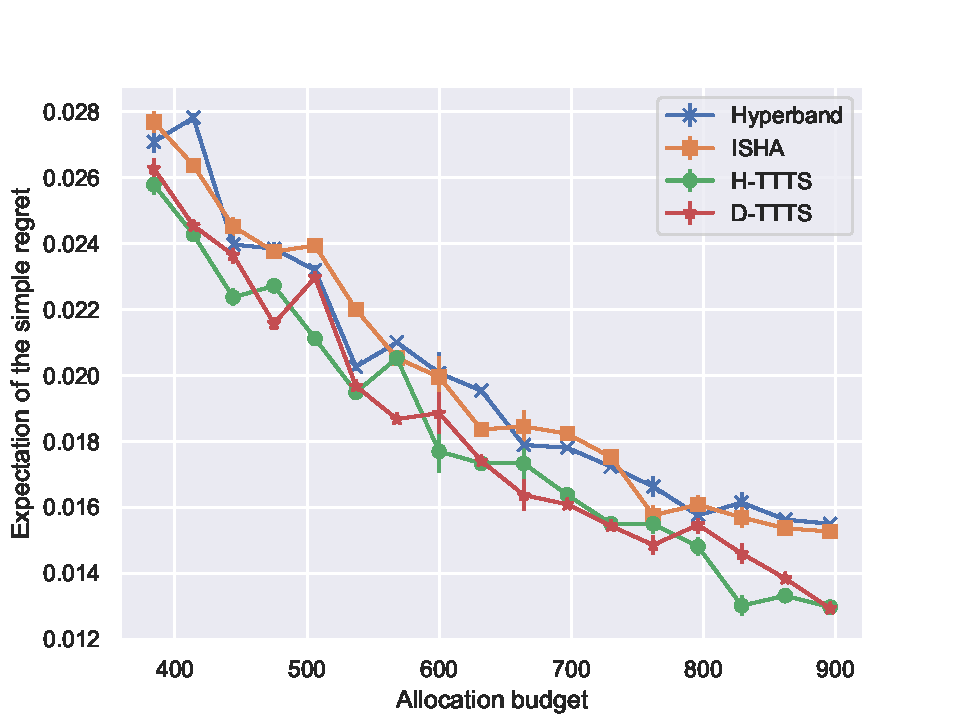
\includegraphics[width=\textwidth]{Chapter6/img/infinite/beta_1_1.pdf}
    \caption{Beta(1,1)}
  \end{subfigure}%
\begin{subfigure}[t]{0.2\textwidth}
    \centering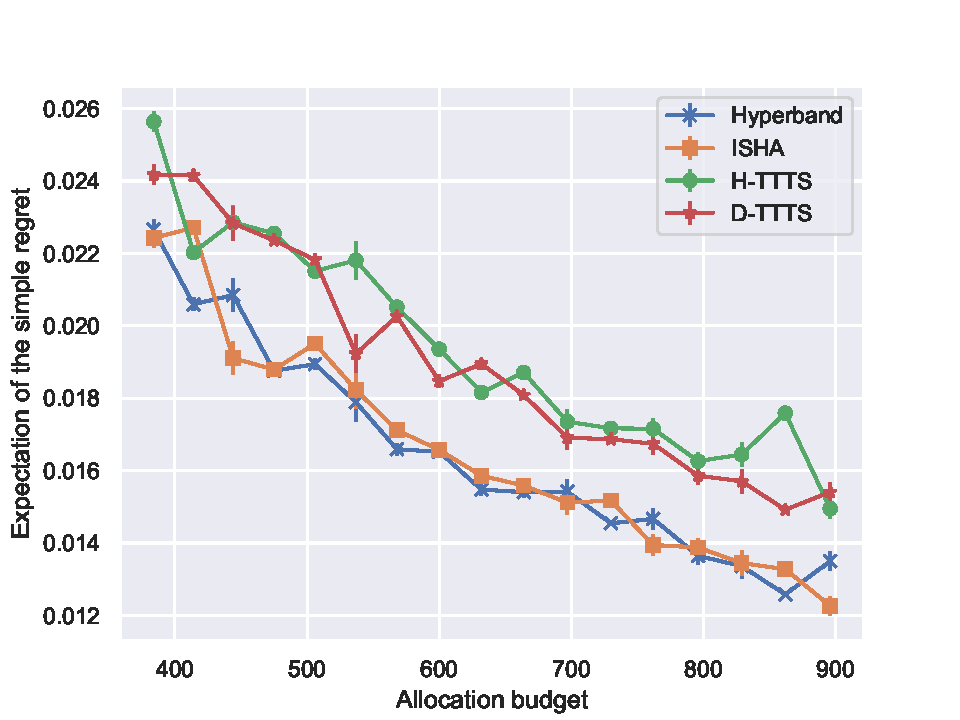
\includegraphics[width=\textwidth]{Chapter6/img/infinite/beta_3_1.pdf}
    \caption{Beta(3,1)}
  \end{subfigure}
  \begin{subfigure}[t]{0.2\textwidth}
    \centering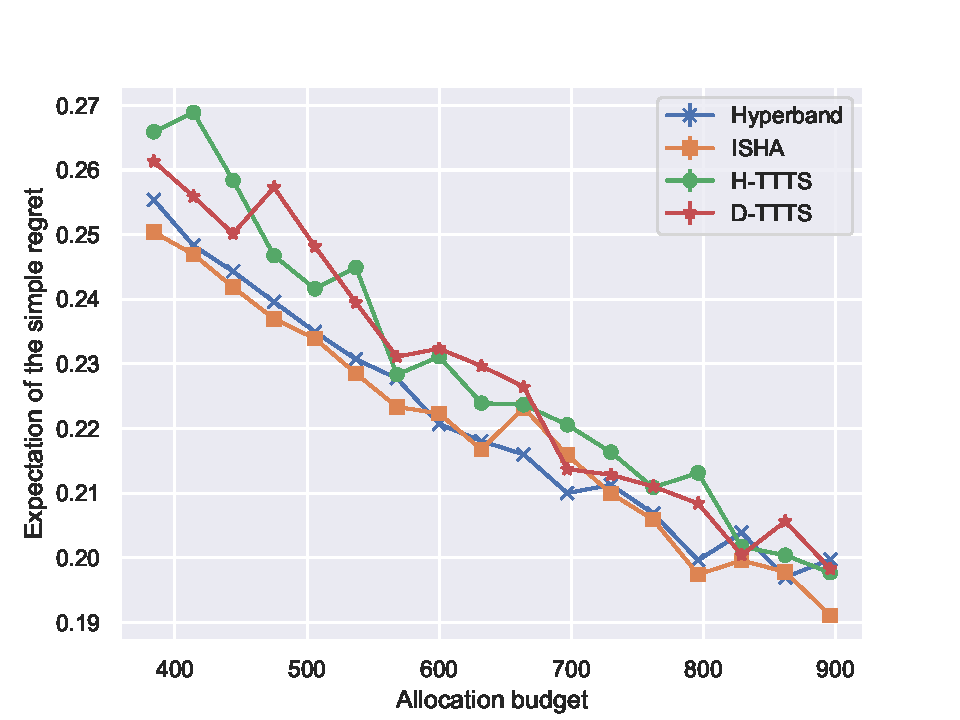
\includegraphics[width=\textwidth]{Chapter6/img/infinite/beta_1_3.pdf}
    \caption{Beta(1,3)}
  \end{subfigure}%
  \begin{subfigure}[t]{0.2\textwidth}
    \centering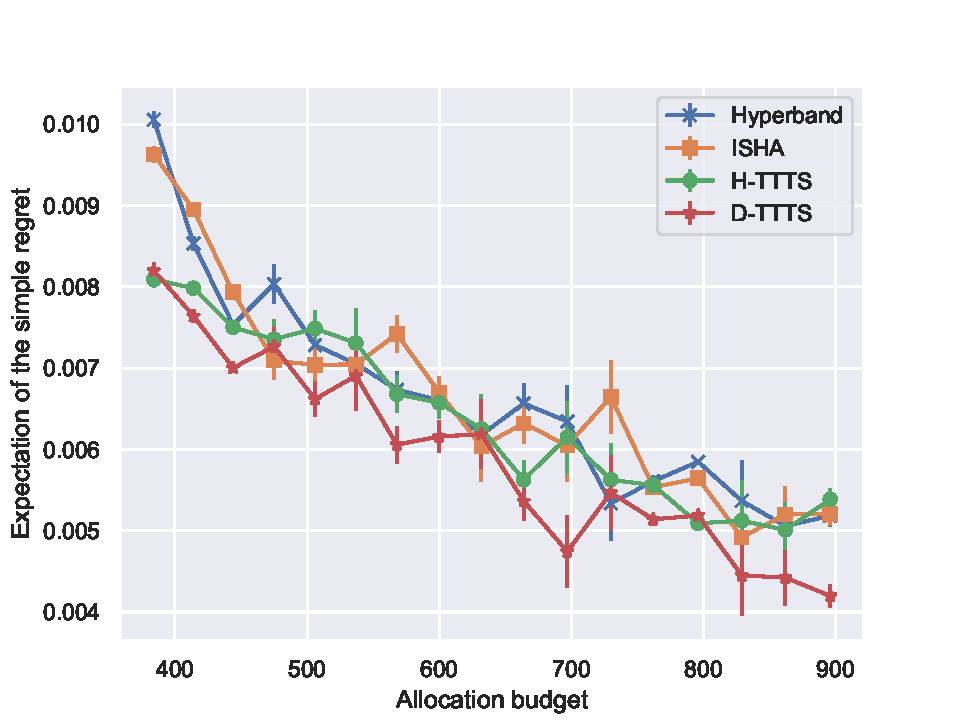
\includegraphics[width=\textwidth]{Chapter6/img/infinite/beta_-5_-5.pdf}
    \caption{Beta(0.5,0.5)}
  \end{subfigure}
  \caption{Simple regret of \DTTTS (against \Hyperband) as a function of the number of arms evaluations for different Beta reservoir.}
  \label{fig:dttts}
\end{figure}

Note that in the implementation of \Hyperband for this \emph{stochastic} infinite bandit setting, the elimination phase of the underlying \texttt{SHA} algorithm is carried out according to the averaged loss of previous samples (as samples from an arm are i.i.d. in this setting and not a converging sequence). In the next section, we apply our algorithm to some real hyper-parameter optimization tasks. 

%\begin{figure}[ht]
%  \centering
%  \begin{subfigure}[t]{0.2\textwidth}
%    \centering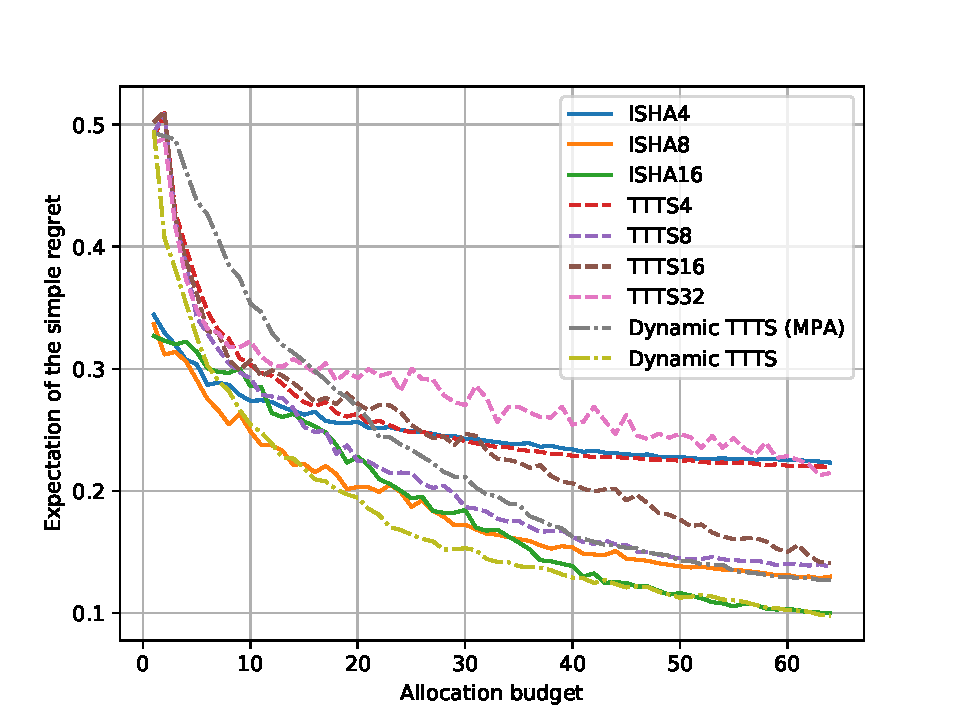
\includegraphics[width=\textwidth]{Chapter6/img/infinite/beta_1_1_64.pdf}
%    \caption{Beta(1,1)}
%  \end{subfigure}%
%  \begin{subfigure}[t]{0.2\textwidth}
%    \centering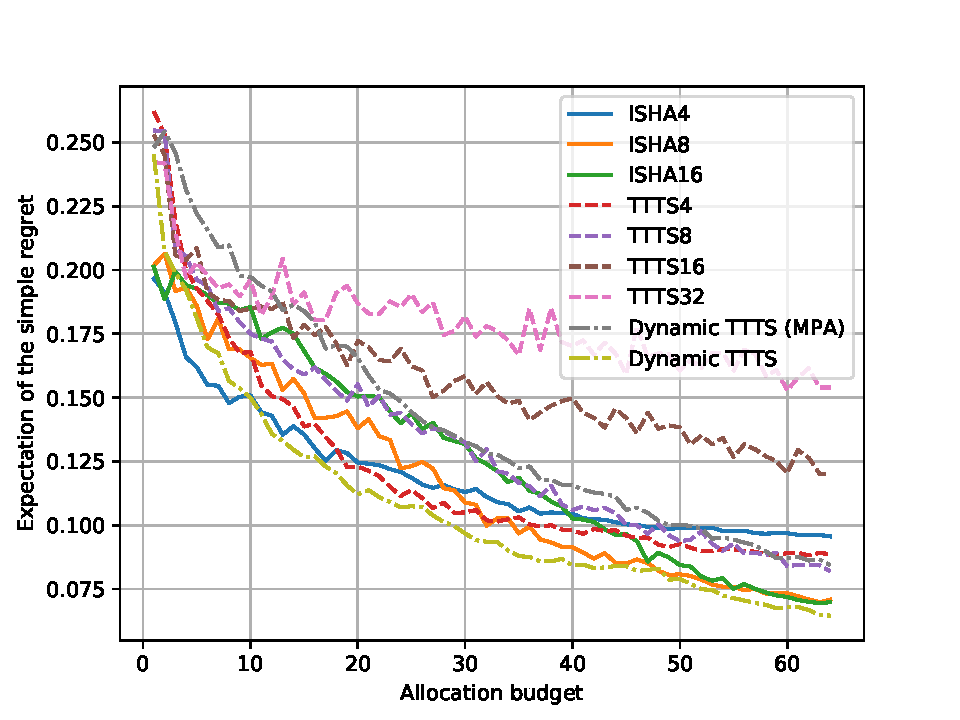
\includegraphics[width=\textwidth]{Chapter6/img/infinite/beta_3_1_64.pdf}
%    \caption{Beta(3,1)}
%  \end{subfigure}
%  \begin{subfigure}[t]{0.2\textwidth}
%    \centering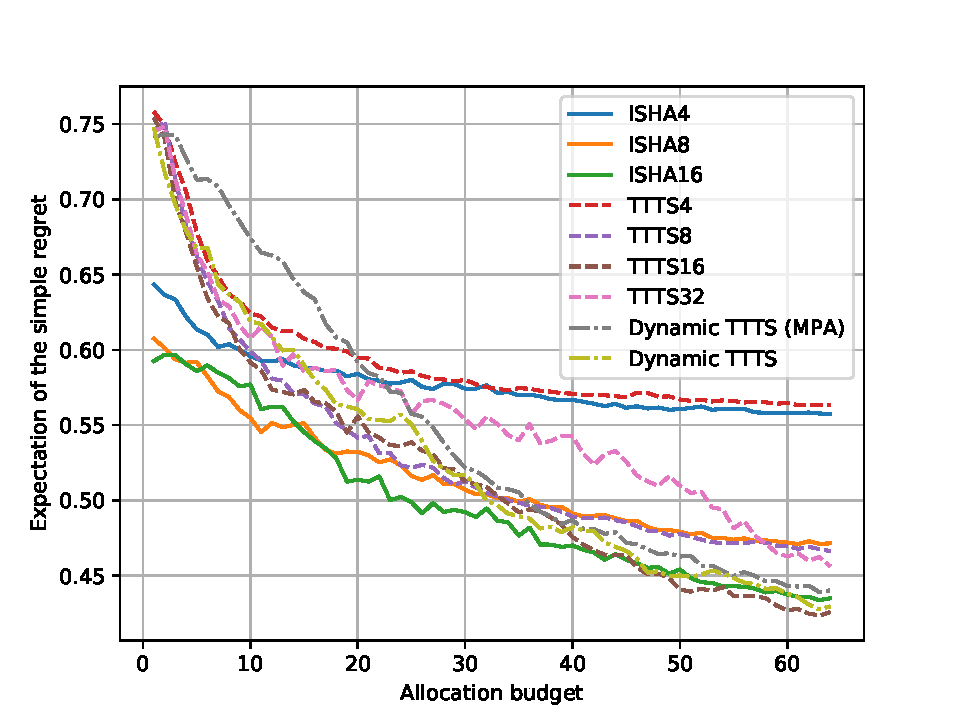
\includegraphics[width=\textwidth]{Chapter6/img/infinite/beta_1_3_64.pdf}
%    \caption{Beta(1,3)}
%  \end{subfigure}%
%  \begin{subfigure}[t]{0.2\textwidth}
%    \centering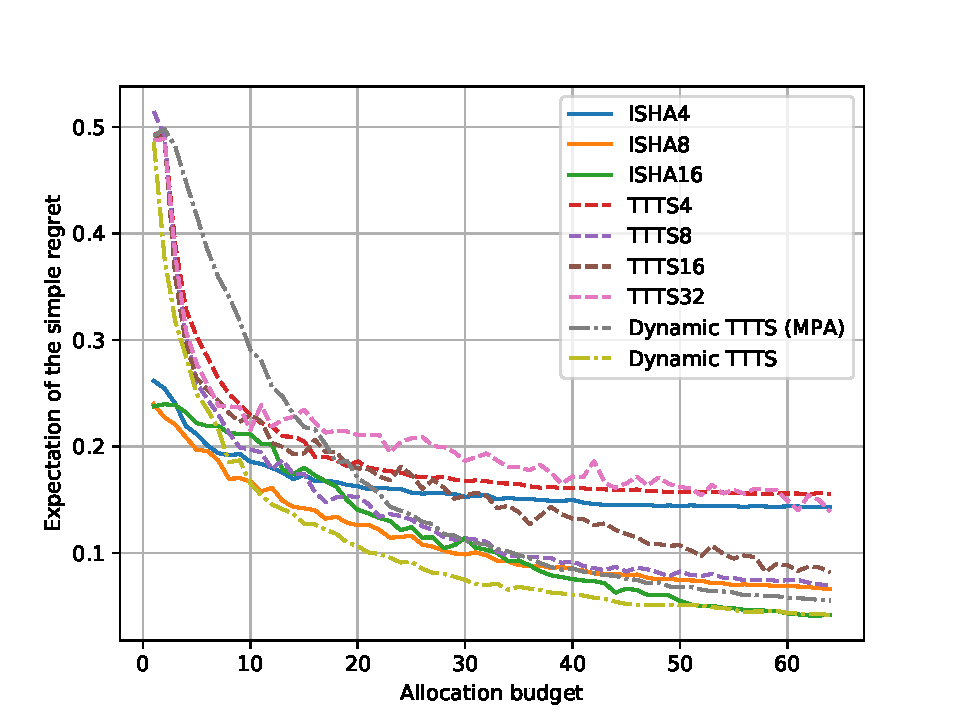
\includegraphics[width=\textwidth]{Chapter6/img/infinite/beta_-5_-5_64.pdf}
%    \caption{Beta(0.5,0.5)}
%  \end{subfigure}
%  %\begin{subfigure}[t]{0.2\textwidth}
%  %  \centering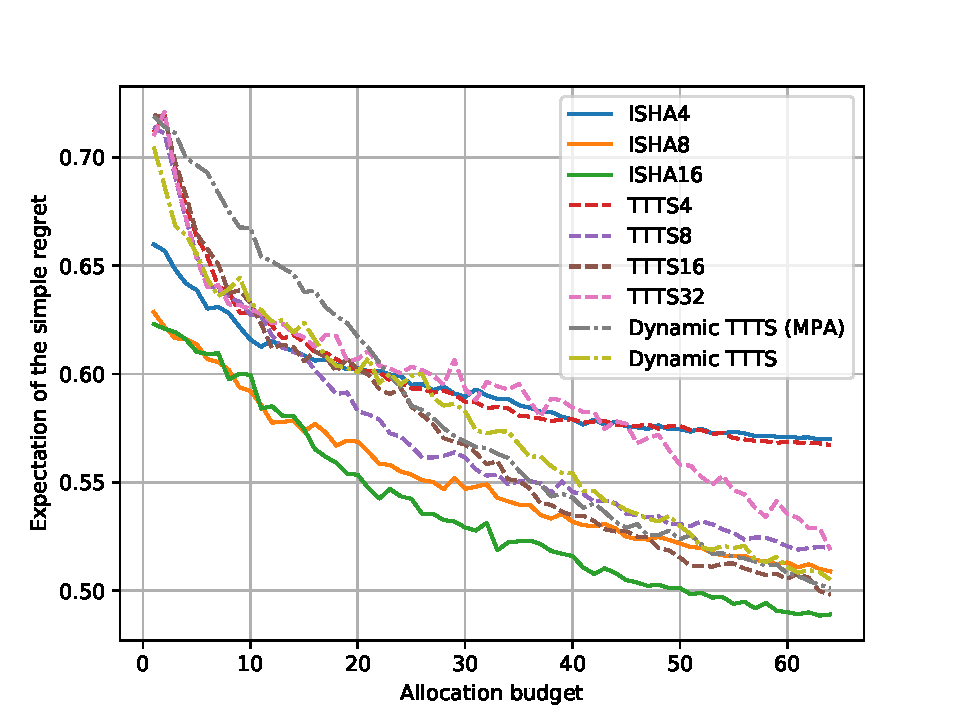
\includegraphics[width=\textwidth]{Chapter6/img/infinite/beta_2_5_64.pdf}
%  %  \caption{Beta(2,5)}
%  %\end{subfigure}
%  %\begin{subfigure}[t]{0.2\textwidth}
%  %  \centering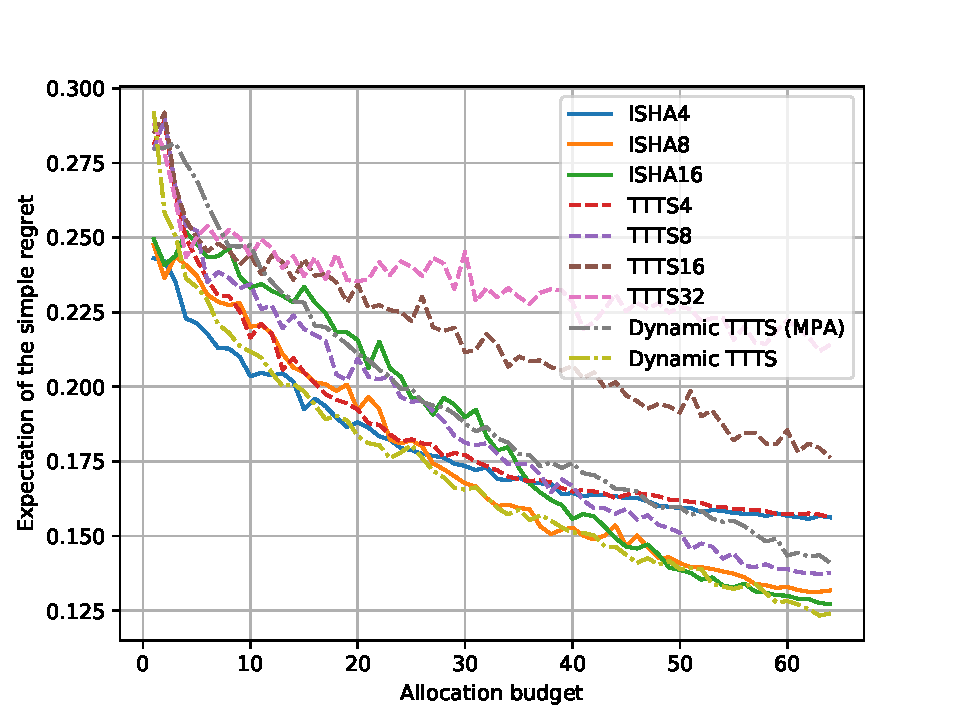
\includegraphics[width=\textwidth]{Chapter6/img/infinite/beta_5_2_64.pdf}
%  %  \caption{Beta(5,2)}
%  %\end{subfigure}
%  %\begin{subfigure}[t]{0.2\textwidth}
%  %  \centering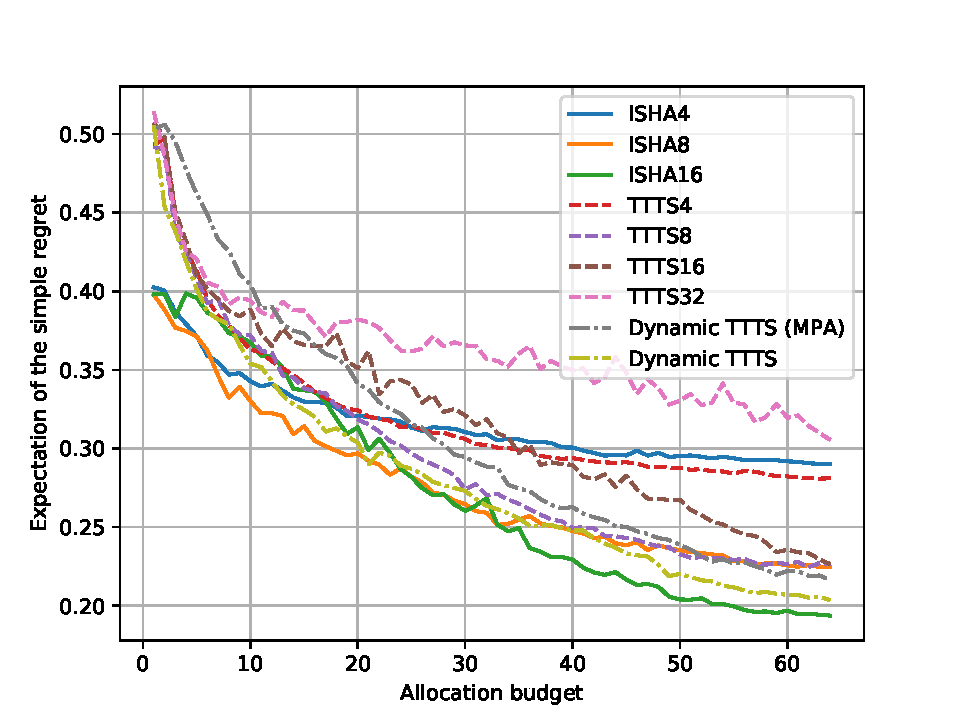
\includegraphics[width=\textwidth]{Chapter6/img/infinite/beta_2_2_64.pdf}
%  %  \caption{Beta(2,2)}
%  %\end{subfigure}
%  %\begin{subfigure}[t]{0.2\textwidth}
%  %  \centering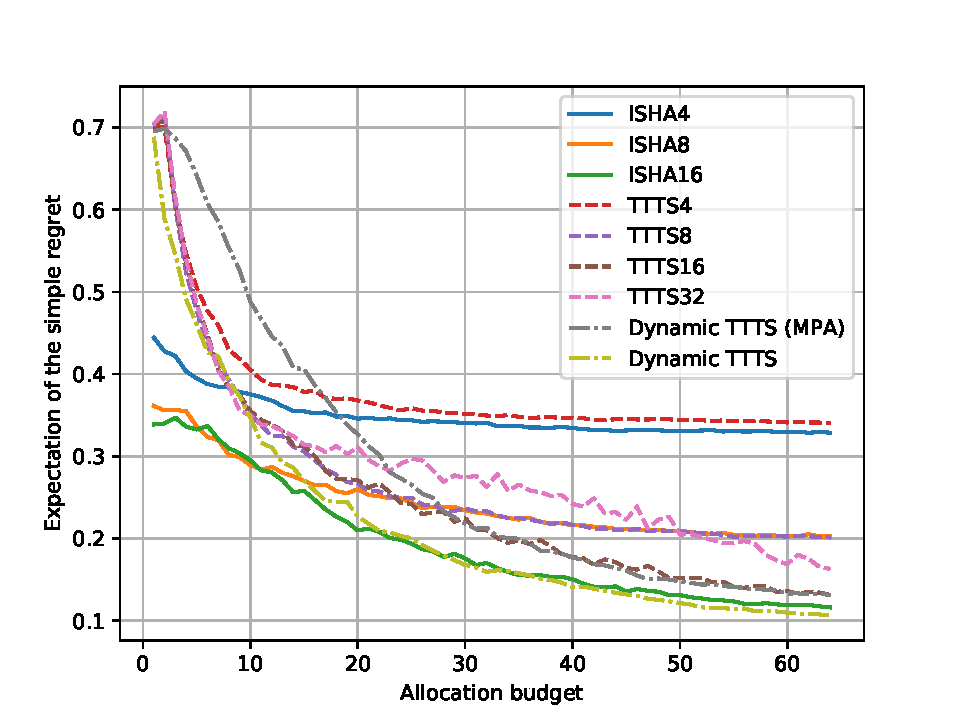
\includegraphics[width=\textwidth]{Chapter6/img/infinite/beta_-3_-7_64.pdf}
%  %  \caption{Beta(0.3,0.7)}
%  %\end{subfigure}
%  \caption{}
%  \label{fig:dttts1}
%\end{figure}
